\documentclass[sigconf, screen, balance=false]{acmart}

\setcopyright{none}
\acmISBN{}
\acmDOI{}
\renewcommand\footnotetextcopyrightpermission[1]{}
\settopmatter{printacmref=false, printfolios=true}

\title{A Technical Overview of the Great Firewall of China}

\author{Shangning Xu}

\begin{document}

\begin{abstract}
    In this paper, we propose a conceptual model of the Great Firewall of China (GFW) as the combination of an IP firewall and an IDS. We also give an overview of its technical capability for censorship based on our conceptual model a review of literature on GFW research.
\end{abstract}

\maketitle

\section{Introduction}

The Great Firewall of China (GFW) is a networking system deployed at nation scale to block access to websites from within China, including popular ones such as Facebook, Google and Instagram. It is of technical interest because of its effectiveness in blocking information access and its capability to handle nation-level network traffic. This paper is organized as follows: We first propose our conceptual model of GFW, then introduce its censorship technical capability based on our conceptual model, and discuss missing research that may be covered in the future.

\section{Conceptual Model}

We view the current iteration of GFW as a combination of an IP firewall and a network-based intrusion detection \& prevention system (IDS), as shown in Figure~\ref{fig:conceptual-model}, where arrows represent information flows. By ``IP firewall'', we mean a router that, in addition to forwarding IP datagrams, may choose to silently drop some datagrams solely based on their IP addresses and static IP address rules. Our definition of an IDS comes from the textbook. An IDS includes multiple \emph{agents} that collect information, a \emph{director} that analyzes collected information to look for threats and signs of intrusion, and a notifier that responds to identified intrusion by sending email notifications or terminating the offending TCP connection, for example. In the case of GFW, rather than looks for signs of intrusion attempts, it looks for signs of offending communication, such as blocked domains, censored keywords, or banned network protocols, and then takes actions to terminate the communication.

\begin{figure}
    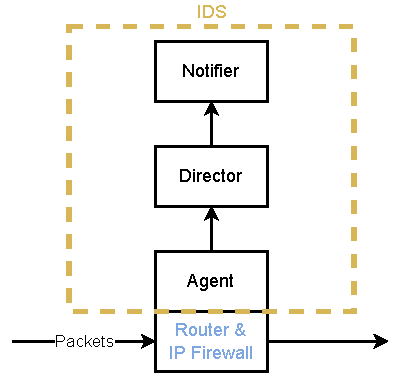
\includegraphics{gfw-node.pdf}
    \caption{Conceptual model of a GFW node}
    \label{fig:conceptual-model}
\end{figure}

Specifying a conceptual model of GFW is important because most people's initial impression of GFW comes from its name: GFW is a firewall. Our conceptual model emphasizes that GFW blocks websites by not only filtering packets, but also actively participating in the communication and injecting new packets. In fact, the latter capability is the primary means through which GFW carries out censorship.

In this model, when a packet arrives at a GFW node, its destination address is matched against the IP blacklist to see whether it should be dropped. If not, a copy of the packet is made and passed to the IDS at upper layers for further analysis, while the original is forwarded correctly towards the destination.

We believe our model closely reflects the reality of GFW for the following reasons:
\begin{itemize}
    \item As will be evident in later sections, it is never observed that GFW can drop packets based on inspection of transport- or application-layer packet data. If the destination IP of a packet is not on the blacklist, GFW can only terminate communication by injecting forged packets that will be sent to the sender and/or the receiver of the offending packet, a form of man-on-the-side attacks.
    \item If packet inspection is involved in the forwarding phase of a router, forwarding will become terribly slow for nation-level or international traffic, leading to congestion at GFW nodes and intolerable delay.
\end{itemize}

The deployment of GFW is symmetric with regard to traffic directions. That is, both inbound (network traffic flowing from to China) and outbound traffic is censored by GFW.

\section{Censorship}

In this section, we describe how GFW censors network communication under our conceptual model of GFW, grouped by network protocols under subsections. The format within each subsection reflects our understanding of GFW as an IDS: we will describe what kinds of information it collects to support its decision, how it decides to censor certain communication and what concrete actions GFW actually takes during censorship. In fact, because our description of censorship is organized by network protocols, each network protocol corresponds exactly to one kind of information GFW collects, thus answering our first question.

\subsection{TCP}

As a transport-layer protocol, a TCP header doesn't carry offending data itself, but the protocol itself is used to actually implement censorship. If after information gathering and analysis, GFW decides to terminate some TCP-based communication like HTTP, it will send TCP RST segments to both parties in the communication, as revealed by \citeauthor{clayton2006ignoring}, one of the earliest research into GFW. \citeauthor{detecting-forged-tcp-reset} fingerprinted TCP RST packets and found multiple RST packets that only appeared in communication involving a Chinese host, likely sent by GFW. They discovered four injectors, differentiated by injected TCP RST packets, and sometimes they operated simultaneously, injecting multiple RST to terminate one TCP connection.

The TCP protocol also present challenges to information gathering and censorship decision of GFW. Due to TCP segmentation and potential packet reordering during network transfer, TCP segments may arrive at a GFW out of order with offending content broken up across two segments. For example, if GFW wishes to scan a TCP connection for the string \texttt{google.com}, instead of one TCP segment that contains the whole string, it may find two TCP segments, with the first one containing \texttt{e.com} and the second \texttt{googl}. To find the offending string, GFW has to reconstruct the TCP flow: sort the segments by their sequence numbers and concatenate TCP payloads. GFW still can't reconstruct TCP flows correctly to this day and segmentation at certain data locations is an effective circumvention strategy employed by \texttt{Geneva} \cite{geneva}, a genetic algorithm that evolves packet manipulation strategies to evade censorship.

\subsection{DNS}

GFW checks the \texttt{QNAME} field in a DNS query message to look for offending host names. Only messages sent from the standard port for DNS (port 53) will experience censorship. \cite{anonymous2020triplet, lowe2007a} \citeauthor{nguyen2021how} identify eight blocking rules in a longitudinal study of GFW's DNS censorship, shown in Table~\ref{tbl:dns-blocking-rules}.

\begin{table}[ht]
    \caption{GFW DNS blocking rules}
    \label{tbl:dns-blocking-rules}
    \begin{tabular}{@{}ll@{}}
        \toprule
        Classification & Patterns \\ \midrule
        Exact Match & \texttt{d} \\
        Prefix & \texttt{d.*},  \texttt{d*} \\
        Suffix & \texttt{*.d}, \texttt{*d} \\
        Mid & \texttt{*.d.*}, \texttt{*.d*}, \texttt{*d.*}, \texttt{*d*} \\
        \bottomrule
    \end{tabular}
\end{table}

These blocking rules are specified with wildcard patterns, where \texttt{*} matches a sequence of characters of \emph{non-zero} length. \texttt{d} is a \emph{base domain} like \texttt{google.com} that GFW wishes to block. For a base domain, only a subset of the identified blocking rules is in effect, and only exact matches trigger censorship. For example, if only the first rule is implemented for the base domain \texttt{google.com}, then the names \texttt{higoogle.com} and \texttt{play.google.com} won't be considered offending because they are not exact matches. These rules are classified by the location of the base domain in the matched host name.

After offending host names are detected, censorship actions depend on the transport-layer protocol of DNS. If TCP is used to transport DNS messages, TCP RST is injected to terminate the TCP connection. \cite{wang2017your} If UDP is used, GFW will reply with forged DNS response messages that contain incorrect IP addresses. For IPv6, all addresses come from the predefined Teredo prefix \texttt{2001::/32}. For IPv4, however, GFW now uses publicly routable IPs owned by foreign entities such as Facebook, WZ Communications Inc., Twitter and Dropbox. \cite{nguyen2021how} The pool of injected IPs evolves from the set of ``bad eight'' \cite{lowe2007a} (eight IP addresses) to its current use of thousands of public routable IPs, which significantly complicates evasion.

Pairing between groups of base domains and injected IP addresses is observed. That is, a set of IP addresses is only injected for a specific group of base domains. \citeauthor{nguyen2021how} identified 11 such pairs or groupings between base domains and injected IP addresses.

Like injection of TCP RST in previous sections, multiple injectors of poisoned DNS response messages are discovered and fingerprinted. \citeauthor{anonymous2020triplet} identified three DNS response injectors, where the most distinctive signature is how IP TTL is set in an IP datagram by each injector: the first injector incremented TTL in successive datagrams, the second used randomized TTL and the third used a fixed TTL. They also discovered that an injector was only responsible for the censorship of a set of base domains and injected a specific group of IPs.

\subsection{HTTP(S)}

In contrast to our discussion of TCP, data carried by the HTTP protocol are analyzed to decide whether to carry out censorship, but the HTTP protocol can't be used to implement censorship. \citeauthor{weinberg2021chinese} conducted a comprehensive test of GFW and showed that it only scanned HTTP GET requests for keywords, specifically the request line that contains the path and the \texttt{Host} header that contains the host name. Censorship was carried out regardless of port numbers, meaning that all port number would be scanned for HTTP requests. They also discovered that if the word \texttt{search} was present in the request line, indicating the HTTP request was sent to a search engine, an \emph{expanded} keyword list would be used in censorship. That is, there were more words that would trigger censorship when the word \texttt{search} was in the request line than it wasn't. GFW used to scan HTTP responses for keywords but ended the practice some time between August 2008 and January 2009, probably due to effectiveness and performance concerns. \cite{park2010empirical}

GFW responds to HTTP GET requests that contain offending keywords with TCP RSTs that are sent to both the client and the server. Residual censorship is observed for the HTTP protocol. Residual censorship refers to the phenomenon that after a communication session between two parties is censored and ends, subsequent communication between the same two parties is subject to stricter, even unconditional censorship. \citeauthor{weinberg2021chinese} reported a 90-second ``penalty box'', during which if the client sends a TCP SYN segment to establish a TCP connection with the same server IP and port number, the GFW will immediately responds with TCP RST to shutdown the connection attempts, regardless of presence of keywords.

As for HTTPS, due to the nature of encryption, GFW can no longer scans the request line for keywords, but it can learn about the website that a client tries to access through the Server Name Identification (SNI) field in the TLS \texttt{ClientHello} message \cite{ChaiGH19}, which is not encrypted. When the first middlebox of GFW detects an offending SNI is detected, it immediately responds with TCP RST immediately. However, if the attempt to terminate the connection is unsuccessful, there is a second middlebox from GFW that will inject another round of TCP RST if the TCP client sends the next packet in TLS handshake: \texttt{ClientKeyExchange} or \texttt{ClientCipherSpec}. \cite{bock2021even} These two messages will trigger censorship even when they don't have the SNI field in them, as long as the previous \texttt{ClientHello} already triggered censorship in the same TCP connection.

The existence of residual censorship for SNI filtering is still in debate. \citeauthor{ChaiGH19} reported a 60-second period of residual censorship, during which ``any SYN packet associated with the 3-tuple (src IP, dst IP, dst port) will trigger a forged SYN/ACK with incorrect sequence number; any other packets will trigger the GFW to send multiple RSTs to both ends.'' \citeauthor{bock2021even} failed to observe residual censorship from the first or the second middlebox.

\subsection{Tor}

The Tor protocol is based on the TLS protocol, and GFW identifies Tor connections by checking the cipher list in the \texttt{ClientHello} message of TLS handshake \cite{wilde2012great}. The cipher suite is unique to Tor and was previously used by Firefox 3. \cite{winter2012how} As an exception to the symmetric censorship on traffic that cross international borders, only outbound traffic \textit{i.e.}, traffic that leaves China is scanned, probably because there is no bridge relay within mainland China through which Tor clients can connect to the Tor network.

When GFW detects Tor traffic, not only does it immediately attempts to terminate the connection by sending TCP RST packets to both the bridge relay and the client, but also follows up by actively probing the server that hosts bridge relay \cite{dunna2018analyzing}. That is, it tries to establish Tor connection with the server on the following range of ports:
\begin{itemize}
    \item Common ports like 80 and 443; and
    \item The port engaged in the previous terminated connection, and its four neighboring ports.
\end{itemize}
After the active scanner completes a successful TLS handshake with any of the port above, GFW confirms that the server is indeed a bridge relay and adds the IP of the bridge relay to the blacklist of the IP firewall, blocking all communication between it and hosts within China. The IP is rescanned every 12 hours and will be removed from the blacklist if the Tor service is no longer running.

\citeauthor{dunna2018analyzing} fingerprinted the active scanners and found that although there was no pattern in IP ID like that reported by TCP RST or DNS response injectors, all packets had a TTL between 48 and 50, a small range of values that suggested these scanners were colocated.

\section{Future Work \& Conclusion}

As with any other research product, this literature review is hopelessly incomplete, and we discuss how our conceptual model can be extended to incorporate future research, both to discuss missing content and to demonstrate our model's extensibility.

First, censorship not covered in this review like \cite{ensafi2015examining} can be discussed under our framework of IDS and classified by network protocols. Our conceptual model of GFW may be refined by works like \cite{anonymous2014towards}, which suggests that the director in our model may actually be a cluster of processors that performs analysis and is connected to multiple agents through a load balancer. Interaction between components may be added \textit{e.g.}, \citeauthor{dunna2018analyzing} suggests that a notifier may add new IPs to the blacklist of the IP firewall.

Even if our model is incomplete in details, we hope it will stand the test of time and become the basis for future research.
\bibliography{ref}
\bibliographystyle{ACM-Reference-Format}

\end{document}
